\EXERCISE
در شکل اول دو درخت دوتایی ریشه‌دار را می‌بینیم که در آن‌ها راسی که حول آن دایره کشیده‌ایم، معرف ریشه است. این درخت‌ها را به دلیل آن که از راس حداکثر دو یال(با نام شاخه) به پایین رسم شده‌اند، دوتایی می‌نامند. این درخت‌های دوتایی مرتب‌اند بدین معنا که شاخه چپی که از راس پایین می‌آید متفاوت از شاخه سمت راستی که از همان راس به پایین می‌آید، در نظر گرفته می‌شود. در حالت وجود
$3$
راس پنج درخت سه‌تایی ریشه‌دار وجود دارد که در شکل دوم نشان داده شده است. تعداد درخت‌های دوتایی ریشه‌دار مرتب با
$n$
راس را پیدا کنید.
\begin{center}
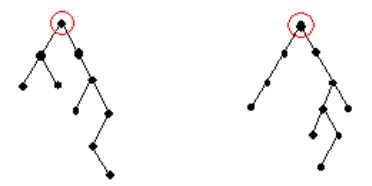
\includegraphics[height=6.5cm]{19.png}
\end{center}
\begin{center}
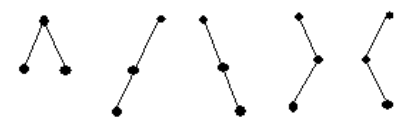
\includegraphics[height=6.5cm]{20.png}
\end{center}